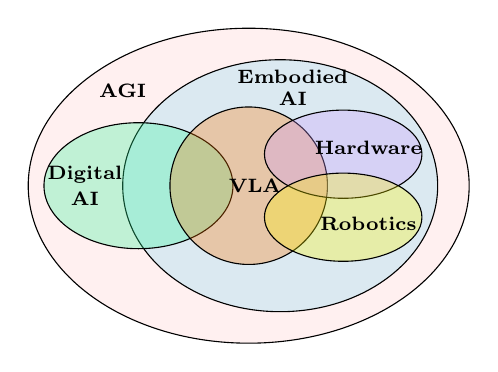
\begin{tikzpicture}[scale=0.8]

    % 设置每个集合的颜色和透明度
    \definecolor{AGI}{RGB}{255, 204, 204}
    \definecolor{EmbodiedAI}{RGB}{137, 221, 246}
    \definecolor{DigitalAI}{RGB}{49, 246, 154}
    \definecolor{VLA}{RGB}{255, 119, 0}
    \definecolor{Hardware}{RGB}{204, 153, 255}
    \definecolor{Robotics}{RGB}{255, 247, 0}

    % 绘制椭圆（请确认颜色名不能有空格）
    \filldraw[fill=AGI, fill opacity=0.3, draw=black] (0.0, 0.0) ellipse (3.5 and 2.5);
    \filldraw[fill=EmbodiedAI, fill opacity=0.3, draw=black] (0.5, 0.0) ellipse (2.5 and 2.0);
    \filldraw[fill=DigitalAI, fill opacity=0.3, draw=black] (-1.75, 0.0) ellipse (1.5 and 1.0);
    \filldraw[fill=VLA, fill opacity=0.3, draw=black, rotate=30] (0.0, 0.0) ellipse (1.25 and 1.25);
    \filldraw[fill=Hardware, fill opacity=0.3, draw=black] (1.5, 0.5) ellipse (1.25 and 0.7);
    \filldraw[fill=Robotics, fill opacity=0.3, draw=black] (1.5, -0.5) ellipse (1.25 and 0.7);

    % 标签
    \node at (-2.0, 1.5) {\scriptsize \textbf{AGI}};
    \node at (0.7, 1.55) {\scriptsize \textbf{\shortstack{Embodied\\AI}}};
    \node at (-2.6, 0.0) {\scriptsize \textbf{\shortstack{Digital\\AI}}};
    \node at (0.1, 0.0) {\scriptsize \textbf{VLA}};
    \node at (1.9, 0.6) {\scriptsize \textbf{Hardware}};
    \node at (1.9, -0.6) {\scriptsize \textbf{Robotics}};

\end{tikzpicture}